% Options for packages loaded elsewhere
\PassOptionsToPackage{unicode}{hyperref}
\PassOptionsToPackage{hyphens}{url}
%
\documentclass[
]{article}
\usepackage{lmodern}
\usepackage{amssymb,amsmath}
\usepackage{ifxetex,ifluatex}
\ifnum 0\ifxetex 1\fi\ifluatex 1\fi=0 % if pdftex
  \usepackage[T1]{fontenc}
  \usepackage[utf8]{inputenc}
  \usepackage{textcomp} % provide euro and other symbols
\else % if luatex or xetex
  \usepackage{unicode-math}
  \defaultfontfeatures{Scale=MatchLowercase}
  \defaultfontfeatures[\rmfamily]{Ligatures=TeX,Scale=1}
\fi
% Use upquote if available, for straight quotes in verbatim environments
\IfFileExists{upquote.sty}{\usepackage{upquote}}{}
\IfFileExists{microtype.sty}{% use microtype if available
  \usepackage[]{microtype}
  \UseMicrotypeSet[protrusion]{basicmath} % disable protrusion for tt fonts
}{}
\makeatletter
\@ifundefined{KOMAClassName}{% if non-KOMA class
  \IfFileExists{parskip.sty}{%
    \usepackage{parskip}
  }{% else
    \setlength{\parindent}{0pt}
    \setlength{\parskip}{6pt plus 2pt minus 1pt}}
}{% if KOMA class
  \KOMAoptions{parskip=half}}
\makeatother
\usepackage{xcolor}
\IfFileExists{xurl.sty}{\usepackage{xurl}}{} % add URL line breaks if available
\IfFileExists{bookmark.sty}{\usepackage{bookmark}}{\usepackage{hyperref}}
\hypersetup{
  pdftitle={How to derive the beautiful probability density function (pdf) of Normal Distribution?},
  pdfauthor={Dan Li},
  hidelinks,
  pdfcreator={LaTeX via pandoc}}
\urlstyle{same} % disable monospaced font for URLs
\usepackage[margin=1in]{geometry}
\usepackage{color}
\usepackage{fancyvrb}
\newcommand{\VerbBar}{|}
\newcommand{\VERB}{\Verb[commandchars=\\\{\}]}
\DefineVerbatimEnvironment{Highlighting}{Verbatim}{commandchars=\\\{\}}
% Add ',fontsize=\small' for more characters per line
\usepackage{framed}
\definecolor{shadecolor}{RGB}{248,248,248}
\newenvironment{Shaded}{\begin{snugshade}}{\end{snugshade}}
\newcommand{\AlertTok}[1]{\textcolor[rgb]{0.94,0.16,0.16}{#1}}
\newcommand{\AnnotationTok}[1]{\textcolor[rgb]{0.56,0.35,0.01}{\textbf{\textit{#1}}}}
\newcommand{\AttributeTok}[1]{\textcolor[rgb]{0.77,0.63,0.00}{#1}}
\newcommand{\BaseNTok}[1]{\textcolor[rgb]{0.00,0.00,0.81}{#1}}
\newcommand{\BuiltInTok}[1]{#1}
\newcommand{\CharTok}[1]{\textcolor[rgb]{0.31,0.60,0.02}{#1}}
\newcommand{\CommentTok}[1]{\textcolor[rgb]{0.56,0.35,0.01}{\textit{#1}}}
\newcommand{\CommentVarTok}[1]{\textcolor[rgb]{0.56,0.35,0.01}{\textbf{\textit{#1}}}}
\newcommand{\ConstantTok}[1]{\textcolor[rgb]{0.00,0.00,0.00}{#1}}
\newcommand{\ControlFlowTok}[1]{\textcolor[rgb]{0.13,0.29,0.53}{\textbf{#1}}}
\newcommand{\DataTypeTok}[1]{\textcolor[rgb]{0.13,0.29,0.53}{#1}}
\newcommand{\DecValTok}[1]{\textcolor[rgb]{0.00,0.00,0.81}{#1}}
\newcommand{\DocumentationTok}[1]{\textcolor[rgb]{0.56,0.35,0.01}{\textbf{\textit{#1}}}}
\newcommand{\ErrorTok}[1]{\textcolor[rgb]{0.64,0.00,0.00}{\textbf{#1}}}
\newcommand{\ExtensionTok}[1]{#1}
\newcommand{\FloatTok}[1]{\textcolor[rgb]{0.00,0.00,0.81}{#1}}
\newcommand{\FunctionTok}[1]{\textcolor[rgb]{0.00,0.00,0.00}{#1}}
\newcommand{\ImportTok}[1]{#1}
\newcommand{\InformationTok}[1]{\textcolor[rgb]{0.56,0.35,0.01}{\textbf{\textit{#1}}}}
\newcommand{\KeywordTok}[1]{\textcolor[rgb]{0.13,0.29,0.53}{\textbf{#1}}}
\newcommand{\NormalTok}[1]{#1}
\newcommand{\OperatorTok}[1]{\textcolor[rgb]{0.81,0.36,0.00}{\textbf{#1}}}
\newcommand{\OtherTok}[1]{\textcolor[rgb]{0.56,0.35,0.01}{#1}}
\newcommand{\PreprocessorTok}[1]{\textcolor[rgb]{0.56,0.35,0.01}{\textit{#1}}}
\newcommand{\RegionMarkerTok}[1]{#1}
\newcommand{\SpecialCharTok}[1]{\textcolor[rgb]{0.00,0.00,0.00}{#1}}
\newcommand{\SpecialStringTok}[1]{\textcolor[rgb]{0.31,0.60,0.02}{#1}}
\newcommand{\StringTok}[1]{\textcolor[rgb]{0.31,0.60,0.02}{#1}}
\newcommand{\VariableTok}[1]{\textcolor[rgb]{0.00,0.00,0.00}{#1}}
\newcommand{\VerbatimStringTok}[1]{\textcolor[rgb]{0.31,0.60,0.02}{#1}}
\newcommand{\WarningTok}[1]{\textcolor[rgb]{0.56,0.35,0.01}{\textbf{\textit{#1}}}}
\usepackage{graphicx}
\makeatletter
\def\maxwidth{\ifdim\Gin@nat@width>\linewidth\linewidth\else\Gin@nat@width\fi}
\def\maxheight{\ifdim\Gin@nat@height>\textheight\textheight\else\Gin@nat@height\fi}
\makeatother
% Scale images if necessary, so that they will not overflow the page
% margins by default, and it is still possible to overwrite the defaults
% using explicit options in \includegraphics[width, height, ...]{}
\setkeys{Gin}{width=\maxwidth,height=\maxheight,keepaspectratio}
% Set default figure placement to htbp
\makeatletter
\def\fps@figure{htbp}
\makeatother
\setlength{\emergencystretch}{3em} % prevent overfull lines
\providecommand{\tightlist}{%
  \setlength{\itemsep}{0pt}\setlength{\parskip}{0pt}}
\setcounter{secnumdepth}{-\maxdimen} % remove section numbering

\title{How to derive the beautiful probability density function (pdf) of
Normal Distribution?}
\author{Dan Li}
\date{2020-08-13}

\begin{document}
\maketitle

How can we derive the probability density function (pdf) of
\textbf{Normal Distribution}?
\[f_Y(y)=\frac{1}{\sqrt{2\pi}\sigma}e^{-\frac{1}{2}(\frac{y-\mu}{\sigma})^2}, \quad -\infty<y<+\infty\]

Let's draw a normal pdf first

\begin{Shaded}
\begin{Highlighting}[]
\CommentTok{\#draw normal pdf}
\NormalTok{x \textless{}{-}}\StringTok{ }\KeywordTok{seq}\NormalTok{(}\OperatorTok{{-}}\DecValTok{5}\NormalTok{, }\DecValTok{5}\NormalTok{, }\DataTypeTok{length.out =} \DecValTok{201}\NormalTok{); dx \textless{}{-}}\StringTok{ }\KeywordTok{diff}\NormalTok{(x)[}\DecValTok{1}\NormalTok{]}
\NormalTok{y \textless{}{-}}\StringTok{ }\KeywordTok{dnorm}\NormalTok{(x, }\DataTypeTok{mean =} \DecValTok{0}\NormalTok{, }\DataTypeTok{sd =} \DecValTok{1}\NormalTok{)}
\NormalTok{base}\OperatorTok{::}\KeywordTok{plot}\NormalTok{(x, y, }\DataTypeTok{type =} \StringTok{"l"}\NormalTok{, }\DataTypeTok{col =} \StringTok{"skyblue"}\NormalTok{,}
           \DataTypeTok{xlab=}\StringTok{"x"}\NormalTok{ , }\DataTypeTok{ylab=}\StringTok{"p(x)"}\NormalTok{ , }\DataTypeTok{cex.lab=}\FloatTok{1.5}\NormalTok{,}
    \DataTypeTok{main=}\StringTok{"Normal Probability Density"}\NormalTok{ , }\DataTypeTok{cex.main=}\FloatTok{1.5}\NormalTok{,}
    \DataTypeTok{lwd=}\DecValTok{2}\NormalTok{)}
\KeywordTok{text}\NormalTok{( }\DecValTok{0}\NormalTok{, }\FloatTok{.6}\OperatorTok{*}\KeywordTok{max}\NormalTok{(y) , }\KeywordTok{bquote}\NormalTok{( }\KeywordTok{paste}\NormalTok{(mu ,}\StringTok{" = 0 "}\NormalTok{) )}
\NormalTok{      , }\DataTypeTok{cex=}\FloatTok{1.5}\NormalTok{ )}
\KeywordTok{text}\NormalTok{( }\DecValTok{0}\NormalTok{, }\FloatTok{.5}\OperatorTok{*}\KeywordTok{max}\NormalTok{(y) , }\KeywordTok{bquote}\NormalTok{( }\KeywordTok{paste}\NormalTok{(sigma ,}\StringTok{" = 1 "}\NormalTok{) )}
\NormalTok{      , }\DataTypeTok{cex=}\FloatTok{1.5}\NormalTok{ )}
\end{Highlighting}
\end{Shaded}

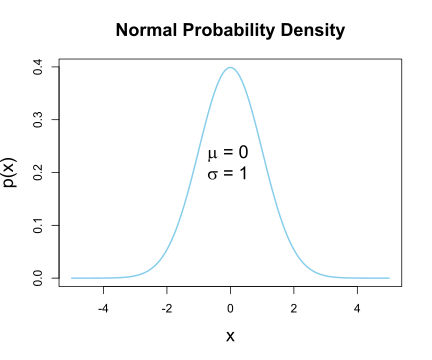
\includegraphics{2020-08-13-distributions_files/figure-latex/unnamed-chunk-1-1.pdf}

\begin{Shaded}
\begin{Highlighting}[]
\KeywordTok{par}\NormalTok{(}\DataTypeTok{mar =} \KeywordTok{c}\NormalTok{(}\DecValTok{4}\NormalTok{, }\DecValTok{4}\NormalTok{, }\DecValTok{2}\NormalTok{, }\FloatTok{.1}\NormalTok{))}
\KeywordTok{curve}\NormalTok{(dnorm, }\DecValTok{{-}3}\NormalTok{, }\DecValTok{3}\NormalTok{, }\DataTypeTok{xlab =} \StringTok{\textquotesingle{}$x$\textquotesingle{}}\NormalTok{, }\DataTypeTok{ylab =} \StringTok{\textquotesingle{}$}\CharTok{\textbackslash{}\textbackslash{}}\StringTok{phi(x)$\textquotesingle{}}\NormalTok{,}
      \DataTypeTok{main =} \StringTok{\textquotesingle{}The density function of $N(0, 1)$\textquotesingle{}}\NormalTok{)}
\KeywordTok{text}\NormalTok{(}\OperatorTok{{-}}\DecValTok{1}\NormalTok{, }\FloatTok{.2}\NormalTok{, }\DataTypeTok{cex =} \DecValTok{3}\NormalTok{, }\DataTypeTok{col =} \StringTok{\textquotesingle{}blue\textquotesingle{}}\NormalTok{,}
  \StringTok{\textquotesingle{}$}\CharTok{\textbackslash{}\textbackslash{}}\StringTok{phi(x)=}\CharTok{\textbackslash{}\textbackslash{}}\StringTok{frac\{1\}\{}\CharTok{\textbackslash{}\textbackslash{}}\StringTok{sqrt\{2}\CharTok{\textbackslash{}\textbackslash{}}\StringTok{pi\}\}e\^{}\{}\CharTok{\textbackslash{}\textbackslash{}}\StringTok{frac\{{-}x\^{}2\}\{2\}\}$\textquotesingle{}}\NormalTok{)}
\end{Highlighting}
\end{Shaded}

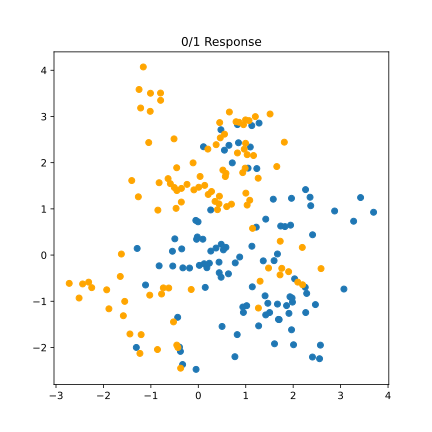
\includegraphics{2020-08-13-distributions_files/figure-latex/unnamed-chunk-2-1.pdf}

Let \(W_1\), \(W_2\), . . . be a set of random variables with mean
\(\mu\) and variance \(\sigma^2\), then \(E(W_i-\mu)=0\),
\(Var(W_i-\mu)=\sigma^2\).

Let \(S_i=(W_i-\mu)/\sigma\), then \(E(S_i)=0\) and \(Var(S_i)=1\), and
then the moment-generating functions of \(S_i\) is \(M(t)\)

Then, \(M_{(S_1+...+S_N)/\sqrt{n}}(t)=[M(t/\sqrt{n})]^n\),

\(M^{(0)}(s)t^0/0!=1\), \(M^{(1)}(s)t^1/1!=E(S_i)t^1/1!=0\),
\(M^{(2)}(s)t^2/2!=M^{(2)}(s)t^2/2\), \ldots\ldots{}
\[M^{(2)}(t/\sqrt{n})t^2/2=M^{(2)}(t)t^2/2n\] When \(n\to+\infty\),
applying Taylor's theorem, for some number r, \textbar r\textbar{}
\textless{} \textbar t\textbar, \[\begin{align}
\lim_{n\to+\infty}[M(t/\sqrt{n})]^n&=\lim_{n\to+\infty}[1+M^{(2)}(r)t^2/2n]^n \\
&=exp\lim_{n\to+\infty}n \;ln[1+M^{(2)}(r)t^2/2n]\\
&=exp\lim_{n\to+\infty}M^{(2)}(r)\frac{t^2}{2}\;\frac{ln[1+M^{(2)}(r)t^2/2n]}{M^{(2)}(r)t^2/2n}\\
&=exp\lim_{n\to+\infty}M^{(2)}(r)\frac{t^2}{2}\;\frac{ln[1+M^{(2)}(r)t^2/2n]-ln(1)}{M^{(2)}(r)t^2/2n}
\end{align}\]

Because as \(n\to+\infty,M^{(2)}(r)\frac{t^2}{2n}\to0\)
\[\lim_{n\to+\infty}\frac{ln[1+M^{(2)}(r)t^2/2n]-ln(1)}{M^{(2)}(r)t^2/2n}=ln^{(1)}1=1\]
Because as \(n\to+\infty,M^{(2)}(r)=Var(S_i)=1\)
\[\lim_{n\to+\infty}M^{(2)}(r)\frac{t^2}{2}=\frac{t^2}{2}\] So,
\[\lim_{n\to+\infty}[M(t/\sqrt{n})]^n=e^{t^2/2}\]

\(e^{\frac{t^2}{2}}\) is the moment-generating function for a standard
normal random variable. So
\(\frac{S_1+...+S_N}{\sqrt{n}}=\frac{W_1+...+W_N-n\mu}{\sqrt{n}\sigma}\)
is a standard normal random variable. Which means
\[\lim_{n\to+\infty}P\Biggl(a\le\frac{W_1+...+W_N-n\mu}{\sqrt{n}\sigma} \le b\Biggl)=\frac{1}{\sqrt{2\pi}}\int_{a}^{b} e^{-z^2/2}dz\]
, which is called \emph{Central Limit Theorem}.

The moment-generating function for a normal random variable Y is:
\[\begin{align}
M_X(t)=E(e^{tY})&=\frac{1}{\sqrt{2\pi}\sigma}\int_{-\infty}^{+\infty}e^{ty} e^{-\frac{1}{2}(\frac{y-\mu}{\sigma})^2}dy\\
&=\frac{1}{\sqrt{2\pi}\sigma}\int_{-\infty}^{+\infty}exp(-\frac{y^2-2y\mu+\mu^2-2\sigma^2ty}{2\sigma^2})dy\\
&=\frac{1}{\sqrt{2\pi}\sigma}\int_{-\infty}^{+\infty}exp(-\frac{(y-(\mu+t\sigma^2))^2-2t\mu\sigma^2-t^2\sigma^4}{2\sigma^2})dy\\
&=\frac{1}{\sqrt{2\pi}\sigma}exp(t\mu+t^2\sigma^2/2)\int_{-\infty}^{+\infty}exp(-\frac{1}{2}\frac{(y-(\mu+t\sigma^2))^2}{\sigma^2})dy\\
&=exp(t\mu+t^2\sigma^2/2)\frac{1}{\sqrt{2\pi}\sigma}\int_{-\infty}^{+\infty}exp\Biggl[-\frac{1}{2}\Bigl[\frac{y-(\mu+t\sigma^2)}{\sigma}\Bigr]^2\Biggr]dy\\
&=e^{t\mu+t^2\sigma^2/2}
\end{align}\]

Let \(Y\) is a normal random variable with mean \(\mu\) and variance
\(\sigma^2\), and let \(W=aY,(a\ne0)\) \(a\) is a constant, then,\\
\[\begin{align}
f_W(\omega)&=\frac{1}{|a|}f_Y(\frac{1}{a}\omega)\\
&=\frac{1}{|a|}\frac{1}{\sqrt{2\pi}\sigma}\int_{-\infty}^{+\infty}e^{-\frac{1}{2}(\frac{\frac{1}{a}y-\mu}{\sigma})^2}dy\\
&=\frac{1}{|a|}\frac{1}{\sqrt{2\pi}\sigma}\int_{-\infty}^{+\infty}e^{-\frac{1}{2}(\frac{y-a\mu}{a\sigma})^2}dy
\end{align}\], which shows that \(W\) is normal random variables with
mean \(a\mu\), variance \(a^2\sigma^2\).

Let \(X\) and \(Y\) are normal random variables with mean \(\mu\) and
variance \(\sigma^2\), and let \(W=X+Y\), then,\\
\[\begin{align}
f_W(w)&=\frac{d}{dw}F_W(w)\\
&=\frac{d}{dw}P(X+Y ≤ w)\\
&=\frac{d}{dw}\Biggl[\int_{-\infty}^{+\infty}\int_{-\infty}^{w-x}f_X(x)f_Y(y)dydx\Biggr]\\
&=\frac{d}{dw}\Biggl[\int_{-\infty}^{+\infty}f_X(x)\Bigl[\int_{-\infty}^{w-x}f_Y(y)dy\Bigr]dx\Biggr]\\
&=\frac{d}{dw}\Biggl[\int_{-\infty}^{+\infty}f_X(x)F_Y(w-x)dx\Biggr]\\
&=\int_{-\infty}^{+\infty}f_X(x)\Biggl[\frac{d}{dw}F_Y(w-x)\Biggr]dx\\
&=\int_{-\infty}^{+\infty}f_X(x)f_Y(w-x)dx\\
&=\int_{-\infty}^{+\infty}\frac{1}{\sqrt{2\pi}\sigma}e^{-\frac{1}{2}(\frac{x-\mu}{\sigma})^2}\frac{1}{\sqrt{2\pi}\sigma}e^{-\frac{1}{2}(\frac{w-x-\mu}{\sigma})^2}dx\\
&=\frac{1}{2\pi\sigma^2}\int_{-\infty}^{+\infty}exp\Biggl[{-\frac{1}{2}\Bigl[(\frac{x-\mu}{\sigma})^2+(\frac{w-x-\mu}{\sigma})^2\Bigr]}\Biggr]dx\\
&=\frac{1}{2\pi\sigma^2}\int_{-\infty}^{+\infty}exp\Biggl[-\frac{1}{2}\frac{(2x^2-2wx+w^2-2w\mu+2\mu^2)}{\sigma^2}\Biggr]dx\\
&=\frac{1}{2\pi\sigma^2}\int_{-\infty}^{+\infty}exp\Biggl[-\frac{1}{2}\frac{(x^2-wx+\frac{1}{2}w^2-w\mu+\mu^2)}{\frac{1}{2}\sigma^2}\Biggr]dx\\
&=\frac{1}{2\pi\sigma^2}\int_{-\infty}^{+\infty}exp\Biggl[-\frac{1}{2}\frac{(x-\frac{1}{2}w)^2+\frac{1}{4}w^2-w\mu+\mu^2)}{\frac{1}{2}\sigma^2}\Biggr]dx\\
&=\frac{1}{\sqrt{2\pi}\sqrt{2}\sigma}exp\Biggl[-\frac{1}{2}\frac{\frac{1}{4}w^2-w\mu+\mu^2}{(\frac{1}{\sqrt{2}}\sigma)^2}\Biggr]
\frac{1}{\sqrt{2\pi}\frac{1}{\sqrt{2}}\sigma}\int_{-\infty}^{+\infty}exp\Biggl[-\frac{1}{2}\frac{(x-\frac{1}{2}w)^2}{(\frac{1}{\sqrt{2}}\sigma)^2}\Biggr]dx\\
&=\frac{1}{\sqrt{2\pi}\sqrt{2}\sigma}exp\Biggl[-\frac{1}{2}\frac{\frac{1}{4}w^2-w\mu+\mu^2}{(\frac{1}{\sqrt{2}}\sigma)^2}\Biggr]\\
&=\frac{1}{\sqrt{2\pi}\sqrt{2}\sigma}exp\Biggl[-\frac{1}{2}\frac{w^2-4w\mu+4\mu^2}{(\sqrt{2}\sigma)^2}\Biggr]\\
&=\frac{1}{\sqrt{2\pi}\sqrt{2}\sigma}exp\Biggl[-\frac{1}{2}\frac{(w-2\mu)^2}{(\sqrt{2}\sigma)^2}\Biggr]
\end{align}\], then \(W=X+Y\) is a new normal random variable with mean
\(2\mu\), variance \(2\sigma^2\).

If \(X\) and \(Y\) are normal random variables with different means
\(\mu_X\) and \(\mu_Y\) and different variances \(\sigma_X^2\) and
\(\sigma_Y^2\), and let \(W=X+Y\), then, \[\begin{align}
f_W(w)&=\frac{1}{\sqrt{2\pi}\sqrt{\sigma_X^2+\sigma_Y^2}}exp\Biggl[-\frac{1}{2}\Bigl[\frac{w-(\mu_X+\mu_Y)}{\sqrt{\sigma_X^2+\sigma_Y^2}}\Bigr]^2\Biggr]
\end{align}\], then \(W=X+Y\) is a new normal random variable with mean
\(\mu_X+\mu_Y\), variance \(\sigma_X^2+\sigma_Y^2\).

If \(X_i, i=1,2,3,...,n\) are \(n\) normal random variables with
different means \(\mu_i\) and different variances \(\sigma_i^2\), and
let \(W=\sum_{i=1}^{n} a_iX_i\), \(a_i\) are constants, then, \(W\) is a
new normal random variable with mean \(\sum_{i=1}^{n}a_i\mu_i\),
variance \(\sum_{i=1}^{n}a_i^2\sigma_i^2\).

\end{document}
